%Theoretical Mechanics Homework_2
\documentclass[10pt,a4paper]{article}
\usepackage[UTF8]{ctex}
\usepackage{bm}
\usepackage{amsmath}
\usepackage{extarrows}
\usepackage{amsthm}
\usepackage{amssymb}
\usepackage{graphicx}
\usepackage{multirow}
\title{理论力学作业\_2}
\author{陈稼霖 \and 45875852}
\date{2018.10.21}
\theoremstyle{remark}
\newtheorem{defi}{Definition}
\newtheorem{cdefi}{\bf 定义}
\begin{document}
\maketitle
\section*{Q1.}解:
如图(\ref{FigureofHomework_2Problem_1}),以水平桌面为原点,与当地敬经线相切的直线为$x$轴,与纬线相切的直线为$y$轴(在图中垂直于纸面,没有标出),垂直于地表向上的直线为$z$轴,建立随桌面绕地轴转动的空间直角坐标系,其中沿$x,y,z$轴的单位矢量分别为$\bm{i},\bm{j},\bm{k}$,设在这一参考系中质点位置坐标为$(x,y,0),$速度的$x,y$ 分量分别为$v_x,v_y$,即$\bm{v} = v_x\bm{i} + v_y\bm{j}$,初始条件下$x = 0, y = 0, v_x = v_{x0}, v_y = v_{y0}$,即$\bm{v}_0 = v_{x0}\bm{i} + v_{y0}\bm{j}$。
\begin{figure}[h]
\centering
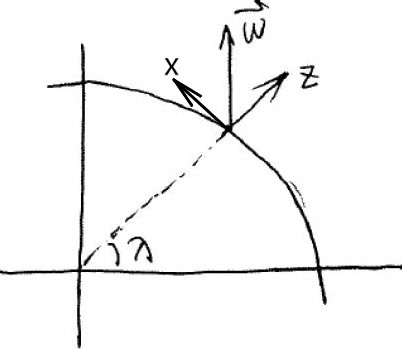
\includegraphics[scale=.6]{FigureofHomework_2Problem_1.jpg}
\caption{Q1图}\label{FigureofHomework_2Problem_1}
\end{figure}

在$O-xyz$转动参考系中,质点受到的离心力包含在重力$mg$中,因为离心力相对于地心引力很小,故可近似认为重力指向地心(沿$z$轴),此外质点还受到桌面垂直于地表的的支持力(沿$z$轴)和垂直于速度方向的科里奥利力
\begin{align*}
-2m\bm{\omega}\times\bm{v} &= -2m(\omega\cos\lambda\bm{i} + \omega\sin\lambda\bm{k})\times(v_x\bm{i} + v_y\bm{j})\\
&= 2m\omega(v_y\sin\lambda\bm{i} - v_x\sin\lambda\bm{j} - v_y\cos\lambda\bm{k})
\end{align*}
根据牛顿第二定律,质点在各轴向上的动力学微分方程为
\begin{align*}
&m\frac{dv_x}{dt} = 2m\omega v_y\sin\lambda\\
&m\frac{dv_y}{dt} = -2m\omega v_x\sin\lambda\\
&m\frac{dv_z}{dt} = F_N - mg - 2m\omega v_y\cos\lambda = 0
\end{align*}
以上三式联立,并考虑初始条件$v_x|_{t = 0} = 0, v_y|_{t = 0} = 0$解得
\begin{align*}
v_x &= v_{x0}\cos(2\omega t\sin\lambda) + v_{y0}\sin(2\omega t\sin\lambda)\\
v_y &= -v_{x0}\sin(2\omega t\sin\lambda) + v_{y0}\cos(2\omega t\sin\lambda)\\
F_N &= m\{g + 2\omega v_y\cos\lambda\}\\
&= m\{g + 2\omega[-v_{x0}\sin(2\omega t\sin\lambda) + v_{y0}\cos(2\omega t\sin\lambda)]\cos\lambda\}
\end{align*}
$v_x, v_y$对时间积分,并考虑初始条件$x|_{t = 0} = 0,y|_{t = 0} = 0$,解得
\begin{align*}
&x = \frac{1}{2\omega\sin\lambda}\{v_{x0}\sin(2\omega t\sin\lambda) + v_{y0}[1 - \cos(2\omega t\sin\lambda)]\}\\
&y = \frac{1}{2\omega\sin\lambda}\{v_{x0}[\cos(2\omega t\sin\lambda) - 1] + v_{y0}\sin(2\omega t\sin\lambda)\}\\
\end{align*}
以上两式联立,消去$t$得到
\[
(v_{x} - \frac{v_{y0}}{2\omega\sin\lambda})^2 + (v_{y} + \frac{v_{x0}}{2\omega\sin\lambda})^2 = \frac{v_{x0}^2 + v_{y0}^2}{4\omega^2\sin^2\lambda}
\]
即
\[
(v_{x} - \frac{v_{y0}}{2\omega\sin\lambda})^2 + (v_{y} + \frac{v_{x0}}{2\omega\sin\lambda})^2 = \frac{v_0^2}{4\omega^2\sin^2\lambda}
\]
故质点的运动轨迹是一个半径为$\frac{v_0}{2\omega\sin\lambda}$的圆。

根据牛顿第三定律,桌面受到的力为
\begin{align*}
\bm{F}_{N}' &= -\bm{F}_{N}= -m\{g + 2\omega v_y\cos\lambda\}\bm{k}\\
&= m\{-g + 2\omega[v_{x0}\sin(2\omega t\sin\lambda) - v_{y0}\cos(2\omega t\sin\lambda)]\cos\lambda\}\bm{k}
\end{align*}
\section*{Q2.}
\subsection*{(i)}解:
如图(\ref{FigureofHomework_2Problem_2}),设$MA = a$,$MB = b$,$\angle OBA = \theta$,$A$点和$B$点坐标$\\((a + b)\sin\theta,0,0)$ 和$(0,(a + b)\cos\theta,0)$,$A$点和$B$点的速度$\bm{v}_A$ 和$\bm{v}_B$,$AB$的角速度$\bm{\omega}$。 分别过$A$点和$B$点作其速度$\bm{v}_A$和$\bm{v}_B$ 的垂线交于$S$ 点,$S$点即为转动瞬心,坐标为$((a + b)\sin\theta,(a + b)\cos\theta,0)$。以椭圆规尺的质心(即$AB$ 的中点)为原点,建立固定在规尺上随规尺运动的直角坐标系$O-x'y'z'$。 取单位矢量$\bm{i},\bm{j},\bm{k}$沿$x$轴,$y$轴和$z$ 轴,单位矢量$\bm{i}',\bm{j}',\bm{k}'$沿$x'$轴,$y'$ 轴和$z'$ 轴。
\begin{figure}[h]
\centering
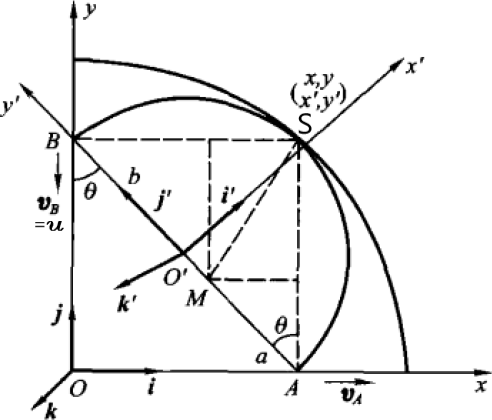
\includegraphics[scale=.5]{FigureofHomework_2Problem_2.png}
\caption{Q2图}\label{FigureofHomework_2Problem_2}
\end{figure}

以$S$点为转轴,$B$点的速率可表示为
\begin{align*}
&v_B = u = (a + b)\sin\theta\cdot\omega\\
&\Longrightarrow\omega = \frac{u}{(a + b)\sin\theta}
\end{align*}
根据转动瞬心的定义,$M$点的速度为
\[
\bm{v}_M = \bm{\omega}\times\overrightarrow{SM} = \omega\bm{k}\times(-a\sin\theta\bm{i}-b\cos\theta\bm{j}) = \frac{u}{(a + b)\sin\theta}(b\cos\theta\bm{i} - a\sin\theta\bm{j})
\]
以$B$为基点,$M$点的加速度为
\begin{align*}
\bm{a}_M &= \bm{a}_B + \frac{d\bm{\omega}}{dt}\times \bm{r}' - \bm{r}'\omega^2 = -\frac{d\omega}{dt}\bm{k}'\times b\bm{j}' + b\omega^2\bm{j}'\\
&= -\frac{d\omega}{d\theta}\frac{d\theta}{dt}\bm{k}'\times b\bm{j}' + b\omega^2\bm{j}'\\
&= -\frac{u\cos\theta}{(a + b)\sin^2\theta}\cdot\omega\cdot b\bm{i}' + b\cot\frac{u^2}{(a + b)^2\sin^2\theta}\bm{j}\\
&= \frac{bu^2}{(a + b)^2\sin^2\theta}(-\frac{\cos\theta}{\sin\theta}\bm{i}' + \bm{j}')\\
&= \frac{bu^2}{(a + b)^2\sin^2\theta}[-\frac{\cos\theta}{\sin\theta}(\cos\theta\bm{i} + \sin\theta\bm{j}) + (-\sin\theta\bm{i} + \cos\theta\bm{j})]\\
&= -\frac{bu^2}{(a + b)^2\sin^2\theta}(\frac{\cos^2\theta}{\sin\theta} + \sin\theta)\bm{i}\\
&= -\frac{bu^2}{(a + b)^2\sin^3\theta}\bm{i}
\end{align*}
\subsection*{(ii)}解:
在固定坐标系$O-xyz$中,设$S$的坐标为$(x,y,z)$,根据(i)中$S$点的坐标为$((a + b)\sin\theta,(a + b)\cos\theta,0)$
\[
\left\{\begin{array}{l}
x = (a + b)\sin\theta\\
y = (a + b)\cos\theta\\
z = 0
\end{array}\right.
\]
消去$\theta$得
\[
\left\{\begin{array}{l}
x^2 + y^2 = (a + b)^2\\
z = 0
\end{array}\right.
\]
故空间极迹为$O-xy$平面上中心在$O$半径等于$(a + b)$的圆周。

在活动系$O'-x'y'z'$中,设$S$的动坐标为$(x',y',z')$,显然$S$点在$O'-x'y'$ 平面上,且$S$点到$O$点距离恒为$\frac{a + b}{2}$,故有
\[
\left\{\begin{array}{l}
x'^2 + y'^2 = [\frac{1}{2}(a + b)]^2\\
z' = 0
\end{array}\right.
\]
故本体极迹方程为$O'-x'y'$平面上中心在$O'$半径等于$\frac{1}{2}(a + b)$ 的圆周。
\section*{Q3.}解:
如图(\ref{FigureofHomework_2Problem_3}),以圆柱体质心为原点建立空间直角坐标系,过原点$O$做$AB$的平行线$CB'$。设圆柱体的密度为$\rho$,则其质量为$m = \pi r^2\cdot2r\rho = 2\pi\rho r^3$。
\begin{figure}[h]
\centering
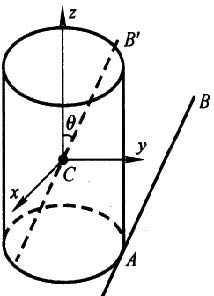
\includegraphics[scale=1]{FigureofHomework_2Problem_3.jpg}
\caption{Q3图}\label{FigureofHomework_2Problem_3}
\end{figure}

先以$CB'$为轴,计算圆柱体的转动惯量:
轴$CB'$对于$x$轴,$y$轴和$z$轴的方向余弦分别为$\alpha = 0, \beta = \sin\theta = \frac{\sqrt{3}}{2}, \gamma = \cos\theta = \frac{1}{2}$;
根据对称性,各惯量积$I_{yz} = I_{zy} = I_{zx} = I_{xz} = I_{xy} = I_{yx} = 0$;各轴转动惯量
\begin{align*}
&I_{xx} = I_{yy} = \int_{-r}^{r}\int_{-\sqrt{r^2 - x^2}}^{\sqrt{r^2 - x^2}}\int_{-r}^{r}(y^2 + z^2)\rho dzdydx = \frac{7}{6}\pi\rho r^5\\
&I_{zz} = \int_{-r}^{r}\int_0^{r}\rho\cdot x^2\cdot2\pi xdxdh = \pi\rho r^5
\end{align*}
故圆柱体对于轴线$A'B'$的转动惯量为
\[
I = I_{xx}\alpha^2 + I_{yy}\beta^2 + I_{zz}\gamma^2 = \frac{9}{8}\pi\rho r^5
\]
再根据平行轴定理计算柱体对于轴线$AB$的转动惯量为
\begin{align*}
I' &= I + m\{\sqrt{r^2 + r^2}\cos[45^{\circ} - (90^{\circ} - \theta)]\}^2\\
&= (\frac{25}{8} + \sqrt{3})\pi\rho r^5\\
&= (\frac{25}{16} + \frac{\sqrt{3}}{2})mr^2
\end{align*}
\subsection*{(ii)}解:
设沿着$x,y,z$轴的单位矢量分别为$\bm{i},\bm{j},\bm{k}$。先求质心$C$ 相对于$A$点的角动量
\begin{align*}
I_C &= \overrightarrow{AC}\times(m\bm{\omega}\times\overrightarrow{AC})\\
&= (-r\bm{j} + r\bm{k})\times[m\omega(\sin\theta\bm{j} + \cos\theta\bm{k})\times(-r\bm{j} + r\bm{k})]\\
&= m\omega r^2(sin\theta + \cos\theta)(\bm{j} + \bm{k})\\
&= \frac{\sqrt{3} + 1}{2}m\omega r^2(\bm{j} + \bm{k})
\end{align*}
柱体相对于$C$点的角动量为
\begin{align*}
J_{C'} &= I_{xx}\bm{\omega_{x}} + I_{yy}\bm{\omega_{y}} + I_{zz}\bm{\omega_{z}}\\
&= \frac{7}{6}\pi\rho r^5\omega\cos\frac{\pi}{2}\bm{i} + \frac{7}{6}\pi\rho r^5\omega\sin\theta\bm{j} + \pi\rho r^5\omega\cos\theta\bm{k}\\
&= \frac{7\sqrt{3}}{12}\pi\rho r^5\omega\bm{j} + \frac{1}{2}\pi\rho r^5\omega\bm{k}
\end{align*}
故柱体相对于$A$点的角动量为
\begin{align*}
J_A &= J_C + J_{C'} = \pi\rho r^5\omega[(\frac{19\sqrt{3}}{12} + 1)\bm{j} + (\sqrt{3} + \frac{3}{2})\bm{k}]\\
&= m\omega r^2[(\frac{19\sqrt{3} + 12}{24})\bm{j} + (\frac{2\sqrt{3} + 3}{4})\bm{k}]
\end{align*}
\section*{Q4.}
\subsection*{(1)}解:
如图(\ref{FigureofHomework_2Problem_4}),以墙角为原点$O$,水平地面为$x$轴,铅锤墙面为$y$轴,建立直角坐标系$O-xy$。设在某一位置时杆与地面所成夹角为$\varphi$,杆与地面和墙面的接触点分别为$A$和$B$,杆的质心为$C$(由于是均质杆,故$C$为$AB$中点),$C$点的速度为$\bm{v}_C$,其$x,y$分量分别为$v_{Cx}$和$v_{Cy}$,杆的角速度为
\begin{figure}[h]
\centering
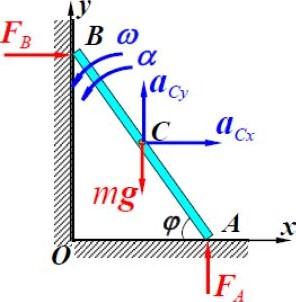
\includegraphics[scale=.6]{FigureofHomework_2Problem_4.jpg}
\caption{Q4图}\label{FigureofHomework_2Problem_4}
\end{figure}

以质心$C$为基点,杆绕$C$点转动的转动惯量为
\[
I = 2\int_0^{\frac{l}{2}}x^2\frac{m}{l}dx = \frac{1}{12}ml^2
\]
根据动能定理有
\[
mg\frac{l}{2}(\sin\varphi_0 - \sin\varphi) = \frac{1}{2}mv_C^2 + \frac{1}{2}I\omega^2
\]
由于$A$点沿着地面运动,故$A$点速度的$y$分量为$0$
\begin{align*}
&v_{Ay} = v_{Cy} + \omega\frac{l}{2}\cos\varphi = 0\\
&\Longrightarrow v_{Cy} = -\omega\frac{l}{2}\cos\varphi
\end{align*}
同理,点$B$沿着墙面运动,故其速度的$x$分量为$0$
\begin{align*}
&v_{Bx} = v_{Cx} - \omega\frac{l}{2}\sin\varphi\\
&\Longrightarrow v_{Cx} = \omega\frac{l}{2}\sin\varphi
\end{align*}
此外,$C$的速度大小与其分量之间的关系为
\[
v_C^2 = v_{Cx}^2 + v_{Cy}^2
\]
以上各式联立,解得杆的角速度为
\[
\omega = \sqrt{\frac{3g}{l}(\sin\varphi_0 - \sin\varphi)}
\]
上式两边同时对$t$求导,得到杆的角加速度为
\[
\beta = \frac{d\omega}{dt} = \sqrt{\frac{3g}{l}}\frac{-cos\varphi}{2\sqrt{\sin\varphi_0 - \sin\varphi}}\frac{d\varphi}{dt} = -\frac{3g}{2l}\cos\varphi
\]
\subsection*{(2)}解:
$C$点速度的$x,y$分量分别为
\begin{align*}
&v_{Cx} = \sqrt{3gl(\sin\varphi_0 - \sin\varphi)}\frac{\sin\varphi}{2}\\
&v_{Cy} = -\sqrt{3gl(\sin\varphi_0 - \sin\varphi)}\frac{\cos\varphi}{2}
\end{align*}
上面两式两边同时对$t$求导,得到$C$点加速度的$x,y$分量为
\begin{align*}
&a_{Cx} = \frac{3g}{2}(\sin\varphi_0 - \frac{3}{2}\sin\varphi)\cos\varphi\\
&a_{Cy} = \frac{3g}{2}[(\sin\varphi_0 - \frac{3}{2}\sin\varphi)\sin\varphi + \frac{1}{2}]
\end{align*}
根据质心运动定理
\begin{align*}
&ma_{Cx} = F_B\\
&ma_{Cy} = F_A - mg
\end{align*}
以上各式联立解得墙壁和地面对杆的约束力分别为
\begin{align*}
&F_B = \frac{3mg}{2}(\sin\varphi_0 - \frac{3}{2}\sin\varphi)\cos\varphi\\
&F_A = \frac{3mg}{2}[(\sin\varphi_0 - \frac{3}{2}\sin\varphi)\sin\varphi + \frac{7}{6}]
\end{align*}
墙壁和地面对杆的约束力的方向分别为水平向右和竖直向上。
\subsection*{(3)}解:
杆脱离墙的那一瞬间,墙壁对杆的约束力恰好为$0$
\[
F_B = \frac{3mg}{2}(\sin\varphi_0 - \frac{3}{2}\sin\varphi)\cos\varphi = 0
\]
解得此时杆与水平面的夹角为
\[
\varphi = \arcsin(\frac{2}{3}\sin\varphi_0)
\]
\section*{Q5.}解:
如图(\ref{FigureofHomework_2Problem_5}),以圆柱体顶点$O$为原点,槽所在直线为$x$轴,在槽和圆锥对称轴所在平面内过$O$点与槽垂直的直线为$y$ 轴,过$O$点垂直于槽和圆锥对称轴所在平面的直线为$z$轴,建立随槽绕圆锥对称轴转动的空间直角坐标系,沿$x,y,z$轴正方向的单位矢量设为$\bm{i},\bm{j},\bm{k}$。设槽对于质点的压力为$\bm{F}_N$,其$y,z$方向分量分别为$F_{Ny},F_{Nz}$
\begin{figure}[h]
\centering
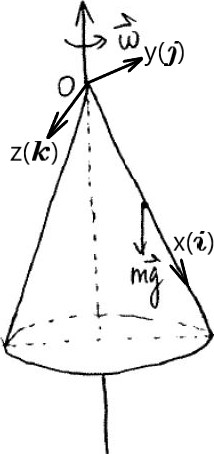
\includegraphics[scale=.6]{FigureofHomework_2Problem_5.jpg}
\caption{Q5图}\label{FigureofHomework_2Problem_5}
\end{figure}

在转动参考系$O-xyz$中,根据牛顿第二定律,质点在各轴向上的动力学微分方程为
\begin{align*}
&m\frac{d^2x}{dt^2} = mg\cos\alpha + m\omega^2 x\sin\alpha\sin\alpha\\
&m\frac{d^2y}{dt^2} = F_{Ny} - mg\sin\alpha + m\omega^2 x\sin\alpha\cos\alpha = 0\\
&m\frac{d^2z}{dt^2} = F_{Nz} + 2m\omega\frac{dx}{dt}\sin\alpha = 0
\end{align*}
以上三式联立,代入$x =s$并考虑初始条件$\left\{\begin{array}{l}x|_{t = 0} = 0\\ \frac{dx}{dt}|_{t = 0} = 0\end{array}\right.$,解得
\begin{align*}
&x = s = \frac{g\cos\alpha}{2\omega^2\sin^2\alpha}(e^{\omega t\sin\alpha} + e^{-\omega t\sin\alpha} - 2)\\
&F_{Ny} = m(g - \omega^2s\cos\alpha)\sin\alpha\\
&F_{Nz} = -2m\omega\sqrt{(2g\cos\alpha + \omega^2s\sin^2\alpha)s}\sin\alpha
\end{align*}
根据牛顿第三定律,质点对槽作用的压力为
\begin{align*}
\bm{F}_{N'} &= -F_{Ny}\bm{j} - F_{Nz}\bm{k}\\
&= m\sin\alpha(\omega^2s\cos\alpha - g)\bm{j} + 2m\omega\sin\alpha\sqrt{(2g\cos\alpha + \omega^2s\sin^2\alpha)s}\bm{k}
\end{align*}
\end{document}
